\documentclass{article}
\usepackage{amsmath}
\usepackage{amssymb}
\usepackage{graphicx}
\usepackage{algorithm}
\usepackage{algpseudocode}
\usepackage{tikz}
\usetikzlibrary{shapes,arrows,positioning,calc}
\usepackage{hyperref}

\title{Methodology: Online 3D Bin Packing with Deep Reinforcement Learning}
\author{}
\date{}

\begin{document}
\maketitle

\section{Introduction}
The Online 3D Bin Packing Problem (3D-BPP) is a fundamental challenge in logistics and supply chain optimization. Unlike its offline counterpart, where all items are known \textit{a priori}, the online variant requires immediate placement decisions for items as they arrive, without knowledge of the future sequence. This constraint significantly increases the complexity, as purely greedy strategies often lead to suboptimal long-term space utilization.

In this work, we propose a Deep Reinforcement Learning (DRL) approach to solve the online 3D-BPP. Our method leverages a Deep Q-Network (DQN) agent that learns to select high-level placement heuristics based on the current state of the container buffer. By integrating a specialized Feasibility Masking mechanism, we prune invalid actions effectively, allowing the agent to focus on learning strategic decision-making policies rather than basic geometric constraints.

\section{Problem Definition}
We define the 3D-BPP as an optimization problem where the objective is to maximize the volumetric utilization of a fixed-size container while satisfying geometric and physical constraints.

\subsection{Mathematical Formulation}
Let the container have dimensions $L \times W \times H$. We consider a sequence of items $B = \{b_1, b_2, \dots, b_N\}$, where each item $i$ has dimensions $(l_i, w_i, h_i)$.
Since the problem is online, the decision for item $i$ must be made at time $i$. However, for theoretical completeness, we model the underlying constraints using a Mixed-Integer Linear Programming (MILP) formulation.

\subsubsection{Decision Variables}
\begin{itemize}
    \item $x_i, y_i, z_i \ge 0$: Coordinates of the front-left-bottom corner of item $i$.
    \item $r_{i} \in \{0, 1\}$: Binary variable indicating rotation (assuming only vertical rotation allowed for simplicity here, i.e., $w$ and $l$ swap).
    \item $p_{ij} \in \{0, 1\}$: Binary variable, 1 if item $i$ is placed in the container, 0 otherwise.
    \item $left_{ij}, right_{ij}, back_{ij}, front_{ij}, under_{ij}, above_{ij} \in \{0, 1\}$: Binary variables ensuring non-overlap between items $i$ and $j$.
\end{itemize}

\subsubsection{Objective Function}
Maximize the total packed volume:
\begin{equation}
    \text{Maximize } \sum_{i=1}^{N} p_{i} \cdot (l_i w_i h_i)
\end{equation}

\subsubsection{Constraints}
\textbf{1. Placement & Dimensions:}
Let effective dimensions be $l'_i, w'_i$.
If $r_i=0$, then $l'_i=l_i, w'_i=w_i$. If $r_i=1$, then $l'_i=w_i, w'_i=l_i$.

\textbf{2. Boundaries:}
\begin{align}
    x_i + l'_i &\le L + M(1-p_i) \\
    y_i + w'_i &\le W + M(1-p_i) \\
    z_i + h_i &\le H + M(1-p_i)
\end{align}

\textbf{3. Non-overlapping:}
For any pair $i, j$ ($i \ne j$), if both are placed ($p_i=1, p_j=1$), at least one relative position must hold:
\begin{equation}
   left_{ij} + right_{ij} + back_{ij} + front_{ij} + under_{ij} + above_{ij} \ge 1
\end{equation}
Implied constraints (e.g., if $left_{ij}=1$, then item $i$ is left of $j$):
\begin{equation}
    x_i + l'_i \le x_j + M(1-left_{ij})
\end{equation}

\textbf{4. Stability (Support Rule):}
Our specific variant enforces a \textbf{coverage constraint}. The area of the base of item $i$ supported by valid surfaces (floor or tops of other items) must be at least 60\%:
\begin{equation}
    Area_{supported}(i) \ge 0.6 \cdot (l'_i \cdot w'_i)
\end{equation}

\section{Reinforcement Learning Structure}
We formulate the problem as a Markov Decision Process (MDP) defined by the tuple $(S, A, R, P, \gamma)$.

\subsection{State Space ($S$)}
The state $s_t$ consists of:
\begin{enumerate}
    \item \textbf{Height Map ($HM$)}: A $L \times W$ grid representing the surface profile.
    \item \textbf{Box Dimensions}: Vector $d_t = (l_t, w_t, h_t)$.
    \item \textbf{Buffer}: Features of the $k$ upcoming items.
\end{enumerate}

\subsection{Action Space ($A$)}
Discrete high-level heuristics:
\begin{itemize}
    \item \textbf{Stacking}: Maximize $z$-coordinate (densify vertical space).
    \item \textbf{Best Fit}: Minimize vertical gap to ceiling.
    \item \textbf{Semi-Perfect Fit}: Minimize local waste + gap.
    \item \textbf{Random Fit}: Stochastic selection.
    \item \textbf{Corner}: Maximize contact with walls/neighbors.
\end{itemize}

\section{Neural Network Architecture}
The agent uses a Dueling DQN architecture with a multi-modal input and an auxiliary mask head.

\begin{figure}[h]
\centering
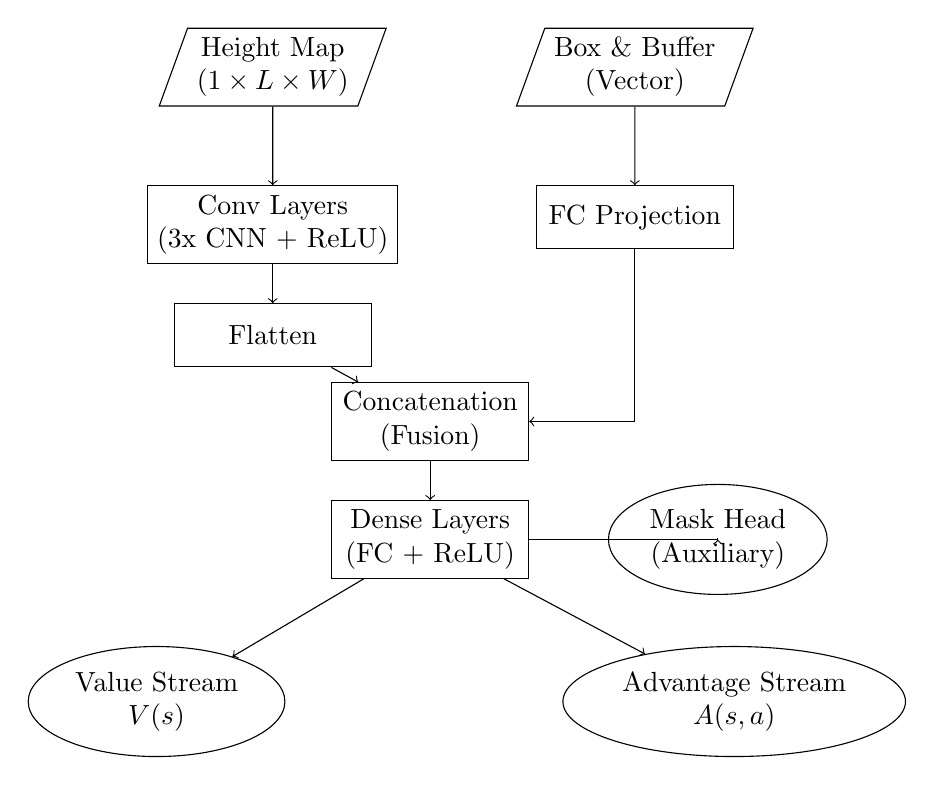
\begin{tikzpicture}[node distance=1cm, auto,
    layer/.style={draw, rectangle, minimum width=2.5cm, minimum height=0.8cm, align=center},
    input/.style={draw, trapezium, trapezium left angle=70, trapezium right angle=110, minimum width=2cm, align=center},
    head/.style={draw, ellipse, minimum width=2cm, align=center}]

    % Inputs
    \node[input] (hm) {Height Map\\($1 \times L \times W$)};
    \node[input, right=2cm of hm] (vec) {Box \& Buffer\\(Vector)};

    % Body
    \node[layer, below=1cm of hm] (conv) {Conv Layers\\(3x CNN + ReLU)};
    \node[layer, below=0.5cm of conv] (flat) {Flatten};
    
    \node[layer, below=1cm of vec] (mlp1) {FC Projection};
    
    % Concatenation
    \node[layer, below=3.5cm of hm, xshift=2cm] (concat) {Concatenation\\(Fusion)};
    
    % Common Tower
    \node[layer, below=0.5cm of concat] (dense) {Dense Layers\\(FC + ReLU)};

    % Heads
    \node[head, below left=1.5cm of dense] (val) {Value Stream\\$V(s)$};
    \node[head, below right=1.5cm of dense] (adv) {Advantage Stream\\$A(s, a)$};
    \node[head, right=1cm of dense] (mask) {Mask Head\\(Auxiliary)};

    % Connections
    \draw[->] (hm) -- (conv);
    \draw[->] (conv) -- (flat);
    \draw[->] (vec) -- (mlp1);
    
    \draw[->] (flat) -- (concat);
    \draw[->] (mlp1) |- (concat);
    
    \draw[->] (concat) -- (dense);
    
    \draw[->] (dense) -- (val);
    \draw[->] (dense) -- (adv);
    \draw[->] (dense) -| (mask);

\end{tikzpicture}
\caption{Dueling DQN Architecture with Auxiliary Mask Head}
\label{fig:nn_arch}
\end{figure}

\section{Experimentation}
\subsection{Synthetic Data Generation (GA Mixer)}
To ensure robustness, we generate training data using a \textbf{Genetic Algorithm (GA)} that mixes episodes from three source distributions:
\begin{itemize}
    \item \texttt{cut\_1} / \texttt{cut\_2}: Variable item counts (11-48), small to large dimensions.
    \item \texttt{rs}: Long random sequences (100 items).
\end{itemize}

\subsubsection{Evolutionary Process}
The GA evolves a population of 2,000 episodes over 60 generations.
\begin{enumerate}
    \item \textbf{Selection}: Tournament selection ($k=3$).
    \item \textbf{Crossover}: \textit{Interleaved Merge}. Two parent episodes combine by strictly alternating items to form a child.
    \item \textbf{Mutation}:
    \begin{itemize}
        \item \textbf{Reorder (15\%)}: Swapping two items within an episode.
        \item \textbf{Switch (10\%)}: Swapping items between different episodes.
        \item \textbf{Dimension (8\%)}: Perturbing $l,w,h$ by $\pm 1$.
    \end{itemize}
    \item \textbf{Fitness}: $F = (1 - |Fill - 0.85|) + \alpha \cdot Diversity$.
\end{enumerate}
This results in the \texttt{ga\_mixed} dataset (10,000 episodes), which balances high fill-rate potential with structural diversity.

\section{Future Developments}
We propose three key directions for future research:

\subsection{Heterogeneous Buffer Management}
Currently, the buffer is passive (FIFO). Future work should explore \textbf{Active Buffer Management}, where the agent learns a policy to decide \textit{which} items to retain in the buffer for long-term utility, effectively learning a "caching" strategy for difficult shapes.

\subsection{Physics-Aware Packing}
Transitioning from simple geometric support constraints to real-time \textbf{Rigid Body Dynamics}. This would account for center-of-mass stability, friction, and item fragility (e.g., heavy items crushing light ones), bridging the gap to real-world robotics.

\subsection{Monte Carlo Tree Search (MCTS) Integration}
Integrating the learned value function $V(s)$ into an MCTS framework during inference. This would allow for a short-term, compute-bounded search to simulate placement consequences before committing, similar to AlphaZero's approach but adapted for the continuous/large discrete space of BPP.

\end{document}
